\documentclass{article}
\usepackage{amsfonts, amsthm, amsmath, amssymb, mathtools, ulem, mathrsfs, physics, esint, siunitx, tikz-cd}
\usepackage{pdfpages, fullpage, color, microtype, cancel, textcomp, markdown, hyperref, graphicx}
\usepackage{enumitem}
\usepackage{algorithm}
\usepackage{algpseudocode}
\graphicspath{{./images/}}
\usepackage[english]{babel}
\usepackage[autostyle, english=american]{csquotes}
\MakeOuterQuote{"}
\usepackage{xparse}
\usepackage{tikz}

\usepackage{calligra}
\DeclareMathAlphabet{\mathcalligra}{T1}{calligra}{m}{n}
\DeclareFontShape{T1}{calligra}{m}{n}{<->s*[2.2]callig15}{}
\newcommand{\script}[1]{\ensuremath{\mathcalligra{#1}}}
\newcommand{\scr}{\script r}

% fonts
\def\mbb#1{\mathbb{#1}}
\def\mfk#1{\mathfrak{#1}}
\def\mbf#1{\mathbf{#1}}
\def\tbf#1{\textbf{#1}}

% common bold letters
\def\bP{\mbb{P}}
\def\bC{\mbb{C}}
\def\bH{\mbb{H}}
\def\bI{\mbb{I}}
\def\bR{\mbb{R}}
\def\bQ{\mbb{Q}}
\def\bZ{\mbb{Z}}
\def\bN{\mbb{N}}

% brackets
\newcommand{\br}[1]{\left(#1\right)}
\newcommand{\sbr}[1]{\left[#1\right]}
\newcommand{\brc}[1]{\left\{#1\right\}}
\newcommand{\lbr}[1]{\left\langle#1\right\rangle}

% vectors
\renewcommand{\i}{\hat{\imath}}
\renewcommand{\j}{\hat{\jmath}}
\renewcommand{\k}{\hat{k}}
\newcommand{\proj}[2]{\text{proj}_{#2}\br{#1}}
\newcommand{\m}[2][b]{\begin{#1matrix}#2\end{#1matrix}}
\newcommand{\arr}[3][\sbr]{#1{\begin{array}{#2}#3\end{array}}}

% misc
\NewDocumentCommand{\seq}{O{n} O{1} O{\infty} m}{\br{#4}_{{#1}={#2}}^{#3}}
\NewDocumentCommand{\app}{O{x} O{\infty}}{\xrightarrow{#1\to#2}}
\newcommand{\sm}{\setminus}
\newcommand{\sse}{\subseteq}
\renewcommand{\ss}{\subset}
\newcommand{\vn}{\varnothing}
\newcommand{\lc}{\epsilon_{ijk}}
\newcommand{\ep}{\epsilon}
\newcommand{\vp}{\varphi}
\renewcommand{\th}{\theta}
\newcommand{\cjg}[1]{\overline{#1}}
\newcommand{\inv}{^{-1}}
\DeclareMathOperator{\im}{im}
\DeclareMathOperator{\id}{id}
\newcommand{\ans}{\tbf{Ans. }}
\newcommand{\pf}{\tbf{Pf. }}
\newcommand{\imp}{\implies}
\newcommand{\impleft}{\reflectbox{$\implies$}}
\newcommand{\ck}{\frac1{4\pi\ep_0}}
\newcommand{\ckb}{4\pi\ep_0}
\newcommand{\sto}{\longrightarrow}
\DeclareMathOperator{\cl}{cl}
\DeclareMathOperator{\intt}{int}
\DeclareMathOperator{\bd}{bd}
\DeclareMathOperator{\Span}{span}
\newcommand{\floor}[1]{\left\lfloor#1\right\rfloor}
\newcommand{\ceil}[1]{\left\lceil#1\right\rceil}
\newcommand{\fxn}[5]{#1:\begin{array}{rcl}#2&\longrightarrow & #3\\[-0.5mm]#4&\longmapsto &#5\end{array}}
\newcommand{\sep}[1][.5cm]{\vspace{#1}}
\DeclareMathOperator{\card}{card}
\renewcommand{\ip}[2]{\lbr{#1,#2}}
\renewcommand{\bar}{\overline}
\DeclareMathOperator{\cis}{cis}
\DeclareMathOperator{\Arg}{Arg}
\newcommand{\ptl}{\partial}

% title
\title{Scientific Computing HW 7}
\author{Ryan Chen}
%\date{\today}
\setlength{\parindent}{0pt}


\begin{document}
	
\maketitle



\tbf{Problem 1.}

\begin{enumerate}[label=(\alph*)]
	
\item Multiplying the BVP by $-1$ and integrating it, we find $k(x)u'=M$ for some constant $M$, i.e. $u'=\frac{M}{k(x)}$. The solution is then
$$u(x) = u_a + \int_a^x \frac{M}{k(s)}ds$$
If $x\le c$ then
$$u(x) = u_a + \int_a^x \frac{M}{k_1}ds = u_a + \frac{M}{k_1}(x-a)$$
If $x>c$ then
$$u(x) = u_a + \int_a^c \frac{M}{k(s)}ds + \int_c^x \frac{M}{k(s)}ds
= u_a + \int_a^c \frac{M}{k_1}ds + \int_c^x \frac{M}{k_2}ds
= u_a + \frac{M}{k_1}(c - a) + \frac{M}{k_2}(x - c)$$
Apply BCs.
$$u_b = u(b)
= u_a + \frac{M}{k_1}(c - a) + \frac{M}{k_2}(b - c)
= u_a + M\sbr{\frac{c-a}{k_1} + \frac{b-c}{k_2}}
\imp M = \frac{u_b-u_a}{\frac{c-a}{k_1}+\frac{b-c}{k_2}}$$
In summary, the solution is
$$u(x) = 
\begin{cases}
	u_a + \frac{M}{k_1}(x-a), & x\le c\\
	u_a + \frac{M}{k_1}(c - a) + \frac{M}{k_2}(x - c), & x>c
\end{cases}
\quad \text{ where }
\quad M = \frac{u_b-u_a}{\frac{c-a}{k_1}+\frac{b-c}{k_2}}$$


\item Given the parameters, it is enough to solve for the values of the 9 mesh points shown below.
\begin{center}
	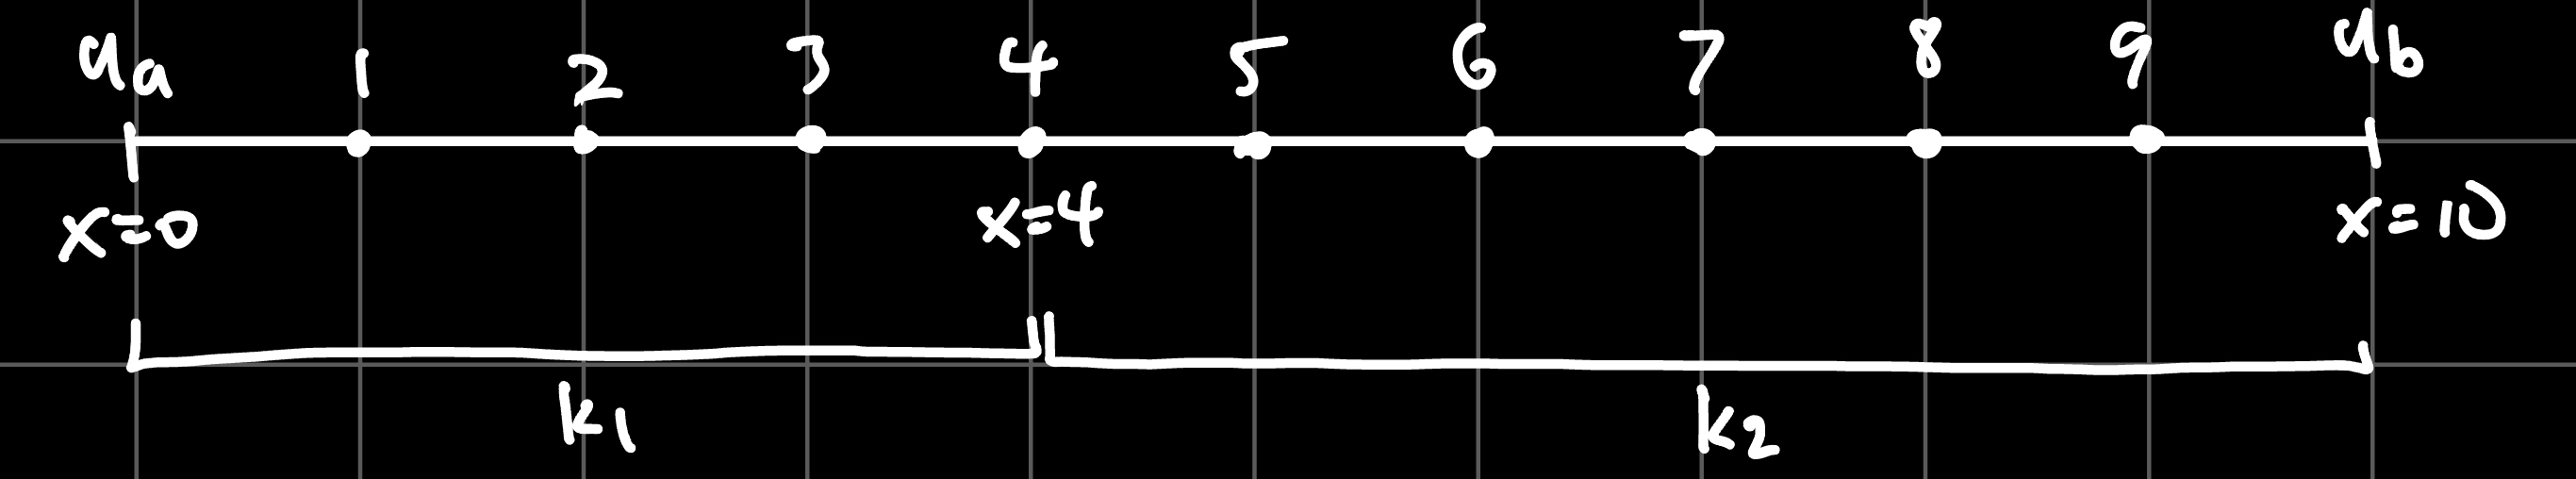
\includegraphics[scale=.09]{hw7 q1 mesh}
\end{center}

The finite difference scheme is
$$L_hu_P = -\frac{1}{h^2}\sbr{k_wu_W + k_eu_E - (k_e + k_w)u_P} = 0
\imp -(k_w + k_e)u_P + k_wu_W + k_eu_E = 0$$
Applying the scheme to each mesh point, we obtain a linear system.
\begin{center}
	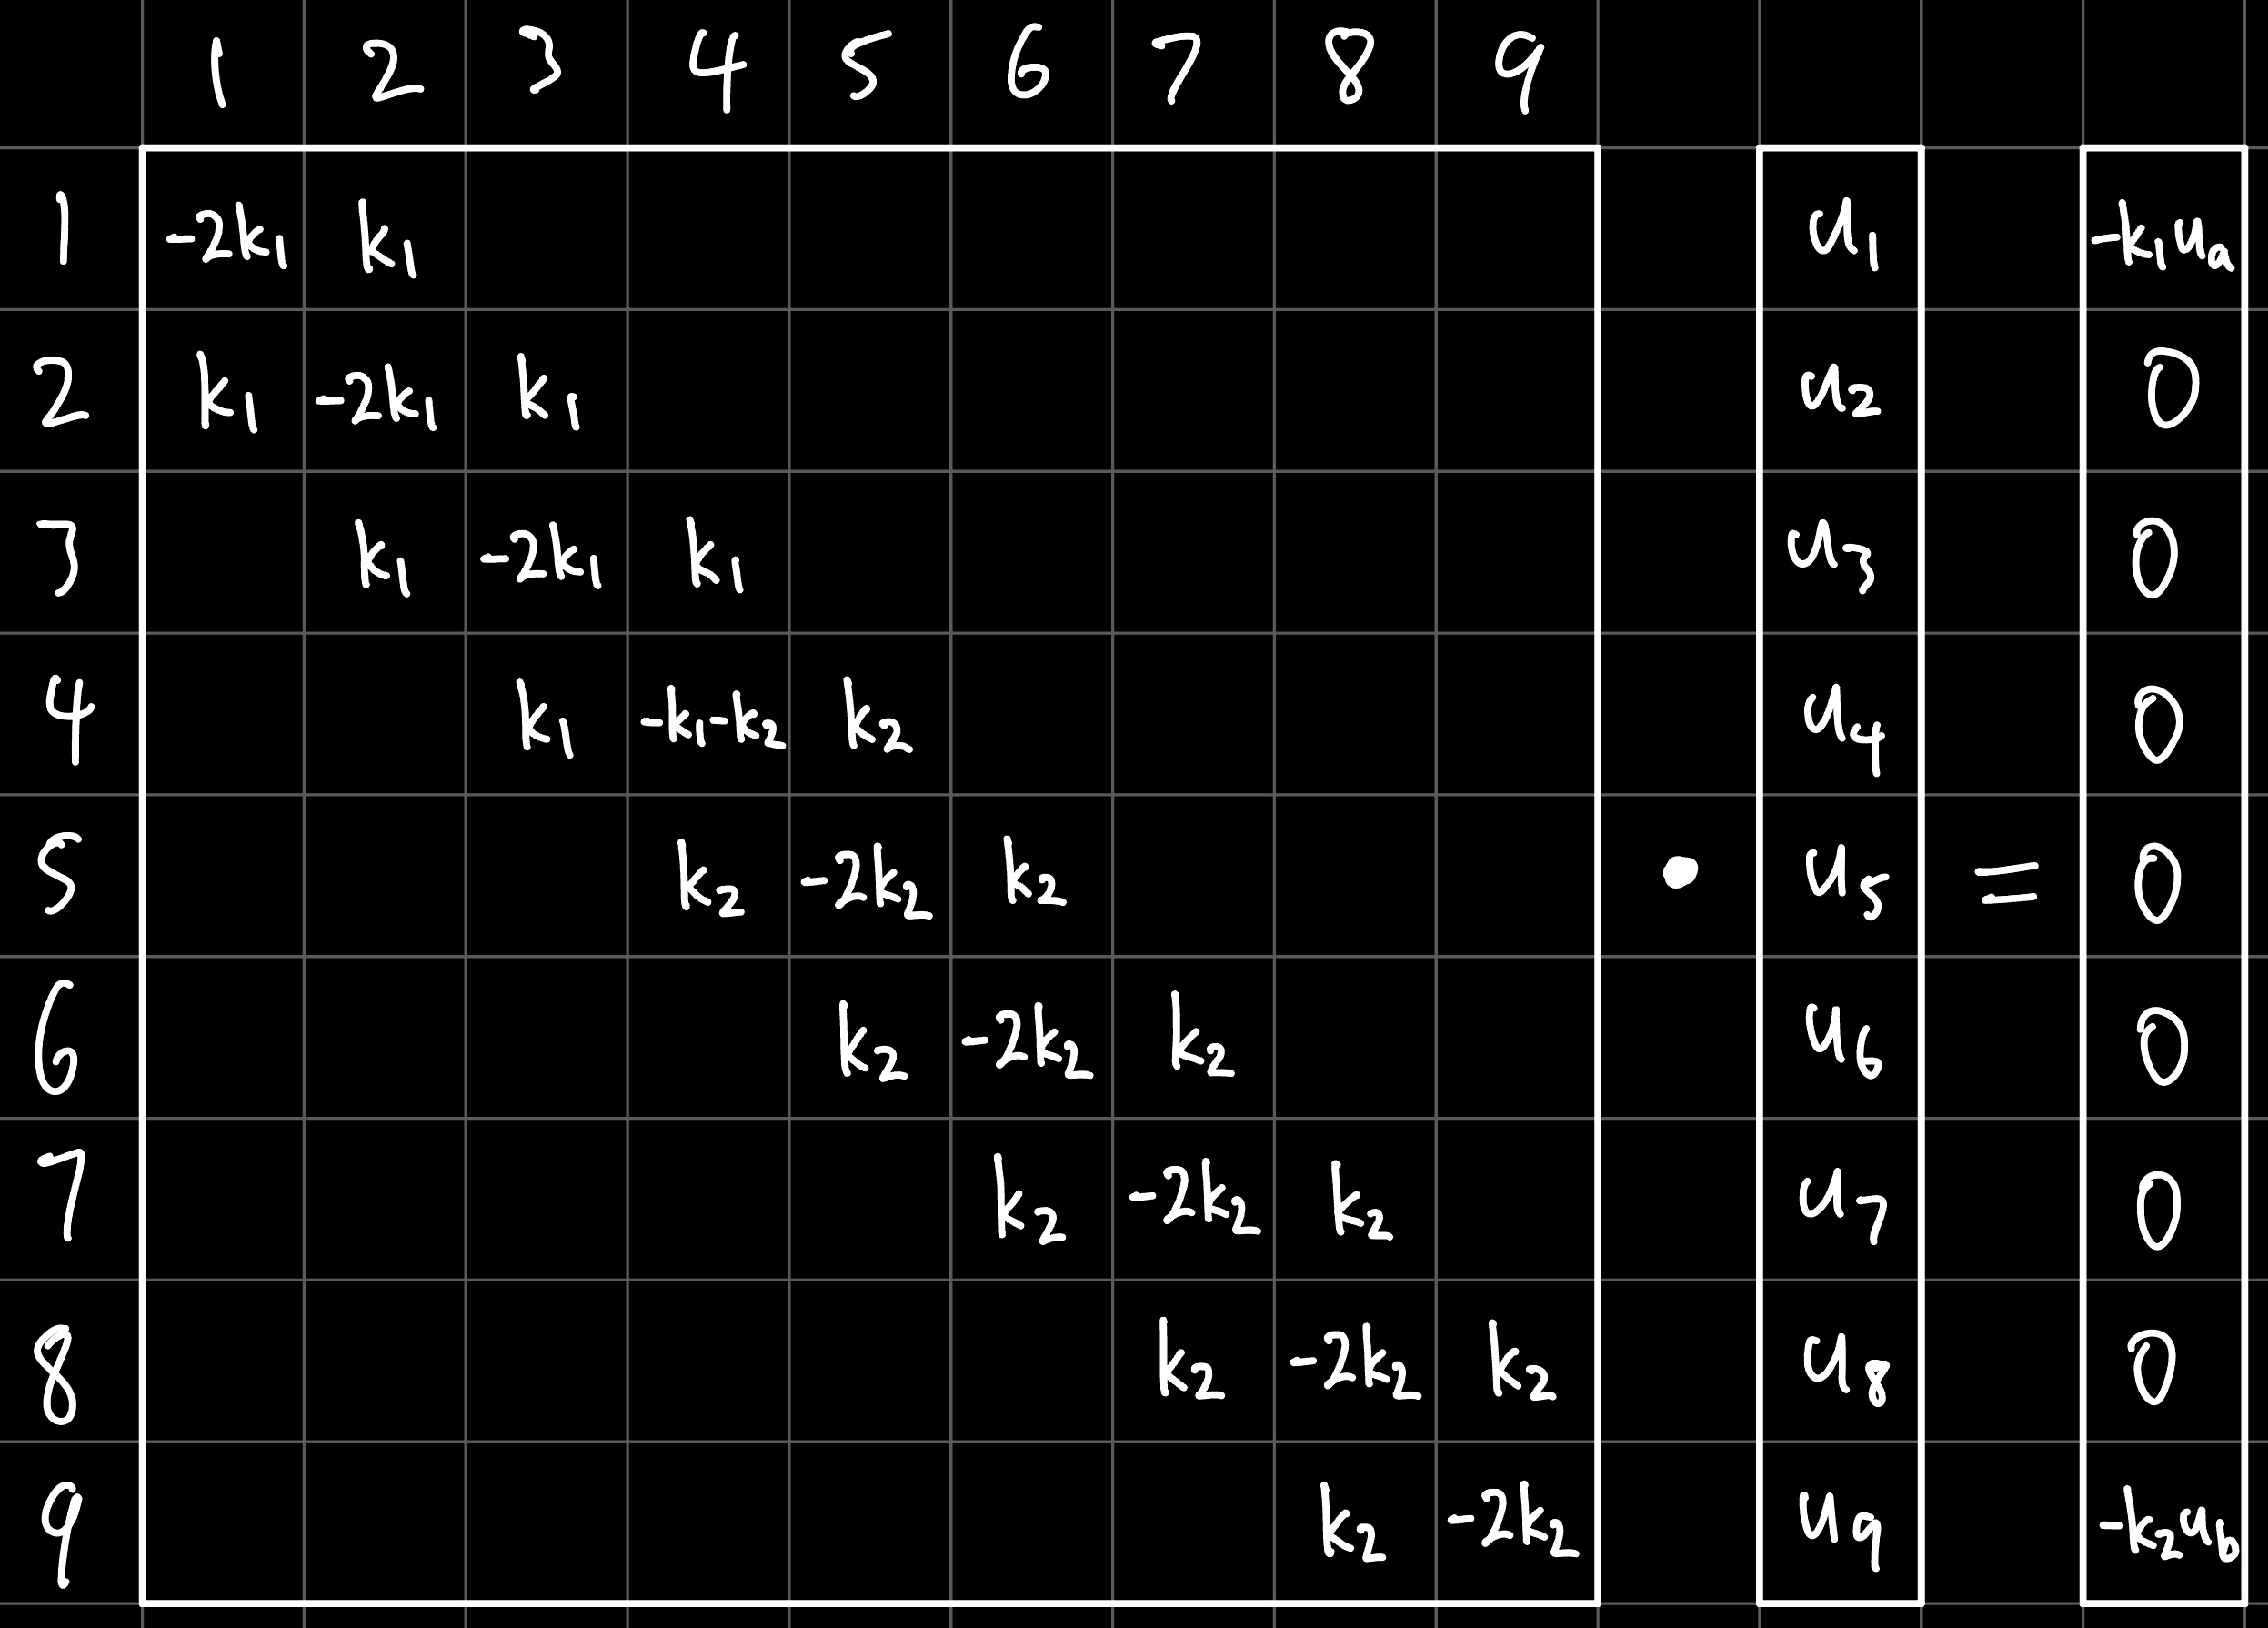
\includegraphics[scale=.09]{hw7 q1 full}
\end{center}

We solve it and plot the numerical solution $u$ along with the exact solution from part (a). In this case the solutions agree exactly.

Code: \url{https://github.com/RokettoJanpu/Scientific-Computing-2/blob/main/hw7q1.ipynb}
\begin{center}
	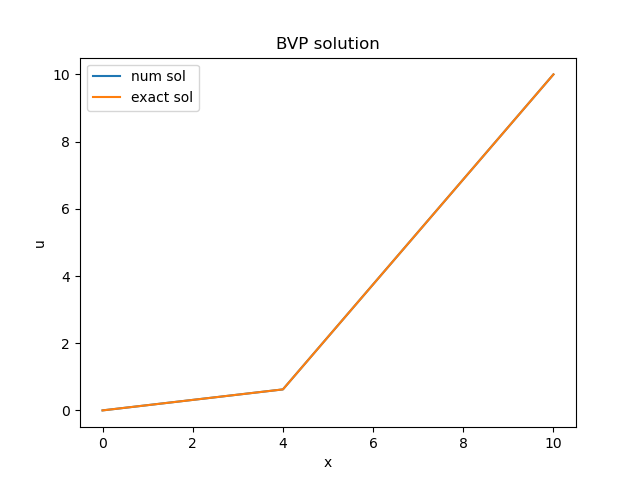
\includegraphics[scale=.5]{hw7 q1 plot}
\end{center}

\end{enumerate}
\sep



\tbf{Problem 2.} Code:

\url{https://github.com/RokettoJanpu/Scientific-Computing-2/blob/main/hw7q2.ipynb}

Below are meshes for the L--shape, the pentagon with a smaller pentagon removed, and the semicircle with two smaller circles removed.

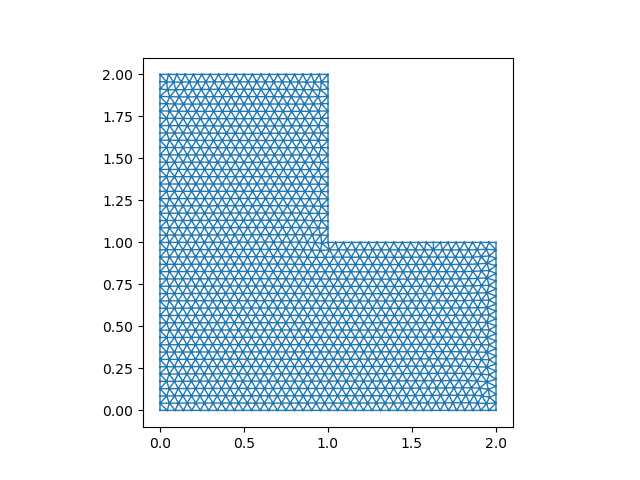
\includegraphics[scale=.35]{hw7 q2 shape 1}
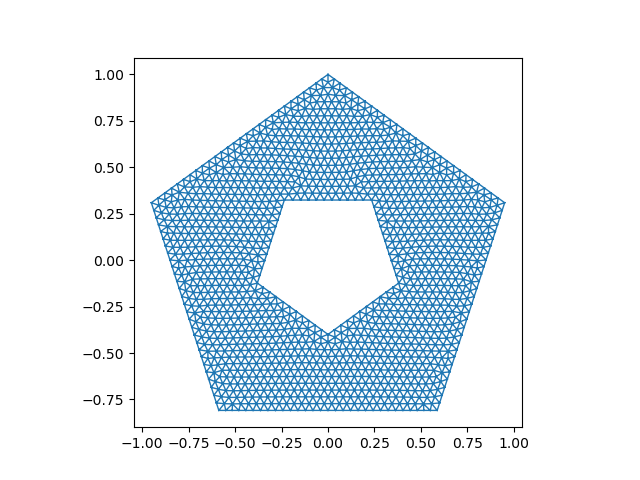
\includegraphics[scale=.35]{hw7 q2 shape 2}
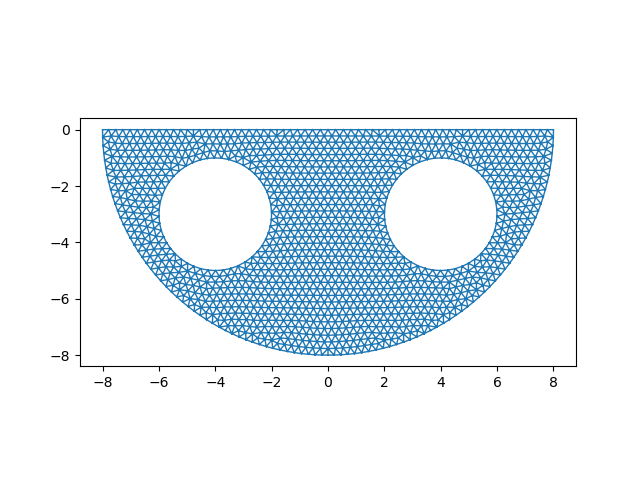
\includegraphics[scale=.35]{hw7 q2 shape 3}
\sep



\tbf{Problem 3.}

\begin{enumerate}[label=(\alph*)]
	
\item Multiply the BVP by $-1$ and multiply by $w$.
$$w(x)u''(x) = -w(x)f(x)$$
Integrate on $[0,1]$. Integrating the LHS by parts, we repeatedly differentiate $w$ and integrate $u$.
\begin{align*}
	\int_0^1 w(x)u''(x)dx &= w(x)u'(x)\eval_0^1 - w'(x)u(x)\eval_0^1 + \int_0^1 w''(x)u(x)dx\\
	&= w(1)u'(1) - w(0)u'(0) - w'(1)u(1) + w'(0)u(0) + \int_0^1 w''(x)u(x)dx\\
	&= -w'(1) + w'(0) + \int_0^1 w''(x)u(x)dx
\end{align*}
We obtain an integral equation for $u$.
$$-w'(1) + w'(0) + \int_0^1 w''(x)u(x)dx = -\int_0^1 w(x)f(x)dx
\imp \int_0^1 w''(x)u(x)dx = -\int_0^1 w(x)f(x)dx + w'(1) - w'(0)$$


\item Fix $1\le i\le N$. The stiffness matrix entries are
$$A_{ij} = \int_0^1\vp_i'(x)\vp_j'(x)dx$$
First compute
$$\vp_i'(x) =
\begin{cases}
	0, & x\le x_{i-1} \text{ or } x\ge x_{i+1}\\
	\frac{1}{x_i-x_{i-1}}, & x_{i-1}<x\le x_i\\
	-\frac{1}{x_{i+1}-x_i}, & x_i<x<x_{i+1}
\end{cases}$$
We examine cases for the value of $j$.

\begin{itemize}
	
	\item If $j\le i-2$ or $j\ge i+2$ then $\vp_i'\vp_j'=0$ hence $A_{ij}=0$.
	
	\item If $j=i-1$ then
	$$\vp_i'(x)\vp_j'(x) =
	\begin{cases}
		0, & x\le x_j \text{ or } x\ge x_i\\
		-\frac{1}{(x_i-x_{i-1})(x_{j+1}-x_j)}, & x_j<x<x_i\\
	\end{cases}$$
	hence
	$$A_{ij} = -\frac{x_i-x_j}{(x_i-x_{i-1})(x_{j+1}-x_j)}$$
	
	\item If $j=i+1$ then
	$$\vp_i'(x)\vp_j'(x) =
	\begin{cases}
		0, & x\le x_i \text{ or } x\ge x_j\\
		-\frac{1}{(x_{i+1}-x_{i})(x_{j}-x_{j-1})}, & x_i<x<x_j\\
	\end{cases}$$
	hence
	$$A_{ij} = -\frac{x_j-x_i}{(x_{i+1}-x_{i})(x_{j}-x_{j-1})}$$
	
	\item If $j=i$ then
	$$\vp_i'(x)\vp_j'(x) =
	\begin{cases}
		0, & x\le x_{i-1} \text{ or } x\ge x_{i+1}\\
		\frac{1}{(x_i-x_{i-1})^2}, & x_{i-1}<x\le x_i\\
		\frac{1}{(x_{i+1}-x_i)^2}, & x_i<x<x_{i+1}
	\end{cases}$$
	hence
	$$A_{ij} = \frac{x_i-x_{i-1}}{(x_i-x_{i-1})^2} + \frac{x_{i+1}-x_i}{(x_{i+1}-x_i)^2}
	= \frac{1}{x_i-x_{i-1}} + \frac{1}{x_{i+1}-x_i}$$
	
\end{itemize}
In summary,
$$A_{ij} = 
\begin{cases}
	0, & j\le i-2 \text{ or } j\ge i+2\\
	-\frac{x_i-x_j}{(x_i-x_{i-1})(x_{j+1}-x_j)}, & j=i-1\\
	-\frac{x_j-x_i}{(x_{i+1}-x_{i})(x_{j}-x_{j-1})}, & j=i+1\\
	\frac{1}{x_i-x_{i-1}} + \frac{1}{x_{i+1}-x_i}, & j=i
\end{cases}$$

\end{enumerate}


\tbf{Problem 4.}

\begin{enumerate}[label=(\alph*)]
	
\item \pf The matrix $G$ is given by
$$G = A\inv \m{0 & 0 \\ 1 & 0 \\ 0 & 1},
\quad A := \m{1 & 1 & 1 \\ x_1 & x_2 & x_3 \\ y_1 & y_2 & y_3}$$
We find $A\inv$ by its adjugate. By cofactor expansion over the first row,
$$D := \det(A)
= \m[v]{x_2 & x_3 \\ y_2 & y_3} - \m[v]{x_1 & x_3 \\ y_1 & y_3} + \m[v]{x_1 & x_2 \\ y_1 & y_2}
= x_2y_3 - x_3y_2 - x_1y_3 + x_3y_1 + x_1y_2 - x_2y_1$$
The matrix of cofactors is
$$\mathrm{cof}(A) = \m{x_2y_3-x_3y_2 & -x_1y_3+x_3y_1 & x_1y_2-x_2y_1 \\ -y_3+y_2 & y_3-y_1 & -y_2+y_1 \\ x_3-x_2 & -x_3+x_1 & x_2-x_1}$$
The adjugate of $A$ is
$$\mathrm{adj}(A) = \mathrm{cof}(A)^T
= \m{x_2y_3-x_3y_2 & -y_3+y_2  & x_3-x_2 \\ -x_1y_3+x_3y_1& y_3-y_1 & -x_3+x_1 \\ x_1y_2-x_2y_1 & -y_2+y_1 & x_2-x_1}$$
Thus
$$G = \frac{1}{D}\mathrm{adj}(A)\m{0 & 0 \\ 1 & 0 \\ 0 & 1}
= \frac{1}{D}\m{y_2-y_3 & x_3-x_2 \\ y_3-y_1 & x_1-x_3 \\ y_1-y_2 & x_2-x_1}$$

Fix an even permutation $(i,j,k)$ of $1,2,3$ (i.e. one of $(1,2,3),~(2,3,1),~(3,1,2)$).
$$\eta_i(x,y) = \frac{\m[v]{1 & x & y \\ 1 & x_j & y_j \\ 1 & x_k & y_k}}{\m[v]{1 & x_i & y_i \\ 1 & x_j & y_j \\ 1 & x_k & y_k}}$$
Since the permutation $(i,j,k)$ is even, the denominator is $\det(A^T)=\det(A)=D$. By cofactor expansion over the first row, the numerator is $x_jy_k - x_ky_j - (y_k - y_j)x + (x_k - x_j)y$, so that
$$\ptl_x\eta_i(x,y) = \frac{1}{D}(y_j-y_k),
\quad \ptl_y\eta_i(x,y) = \frac{1}{D}(x_k-x_j)$$
Thus
$$\m{\ptl_x\eta_1(x,y) & \ptl_y\eta_1(x,y) \\ \ptl_x\eta_2(x,y) & \ptl_y\eta_2(x,y) \\ \ptl_x\eta_3(x,y) & \ptl_y\eta_3(x,y)}
= \frac{1}{D}\m{y_2-y_3 & x_3-x_2 \\ y_3-y_1 & x_1-x_3 \\ y_1-y_2 & x_2-x_1}
= G$$


\item Using the functions $\eta_j$ from (a) and the fact $\grad\eta_j$ is the $j$th row of $G$,
$$u(x,y) = \sum_{j=1}^3 u_j\eta_j(x,y)
\imp \grad u(x,y) = \sum_{j=1}^3 u_j \grad\eta_j(x,y)
= \frac{1}{D}\br{u_1\m{y_2-y_3 \\ x_3-x_2} + u_2\m{y_3-y_1 \\ x_1-x_3} + u_3\m{y_1-y_2 \\ x_2-x_1}}$$
$$\imp \grad u(x,y) = (x_2y_3 - x_3y_2 - x_1y_3 + x_3y_1 + x_1y_2 - x_2y_1)\inv\m{u_1(y_2-y_3)+u_2(y_3-y_1)+u_3(y_1-y_2) \\ u_1(x_3-x_2)+u_2(x_1-x_3)+u_3(x_2-x_1)}$$

\end{enumerate}
	
\end{document}